\chapter{Delhi et mariage indien}
\section*{19 décembre 2015}
Je suis invité à côté de Delhi par des amis, Isabelle et Vijay dont le frère va se marier \newline
 Une journée de visite de la capitale indienne, plongée en permanence dans un brouillard de pollution \newline
 \newline
\centerline{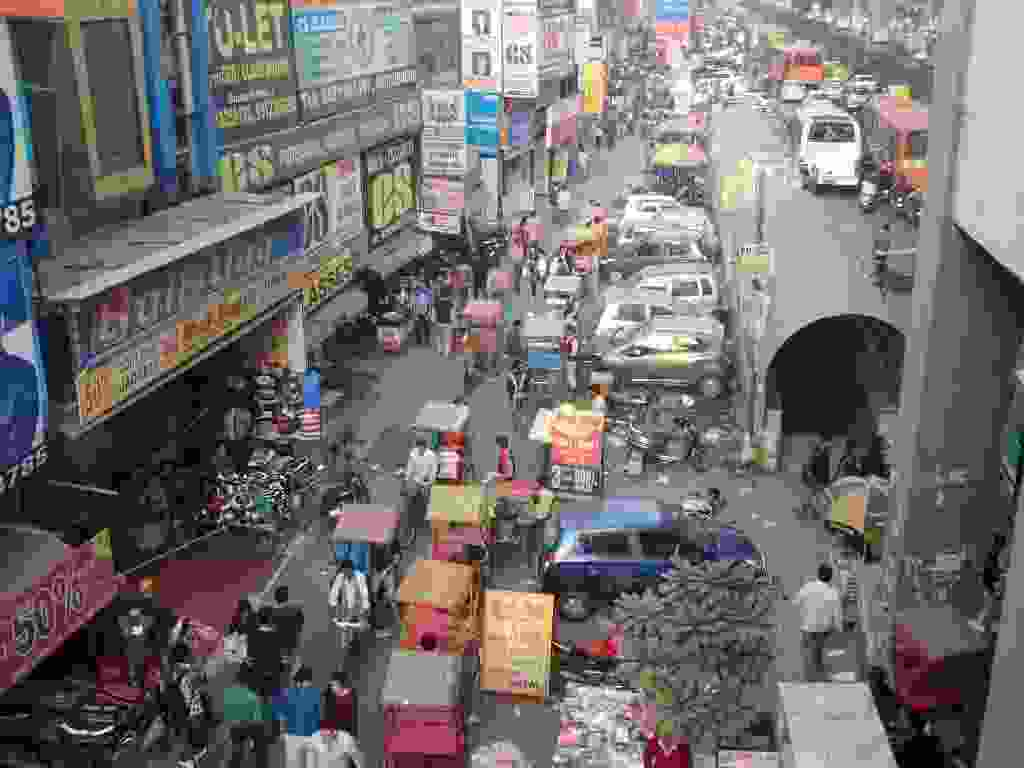
\includegraphics[height=90mm]{../wp-content/uploads/2015/12/wpid-oi0005542-1024x768.jpg} } 
 \newline
 Place Connaugh \newline
 \newline
\centerline{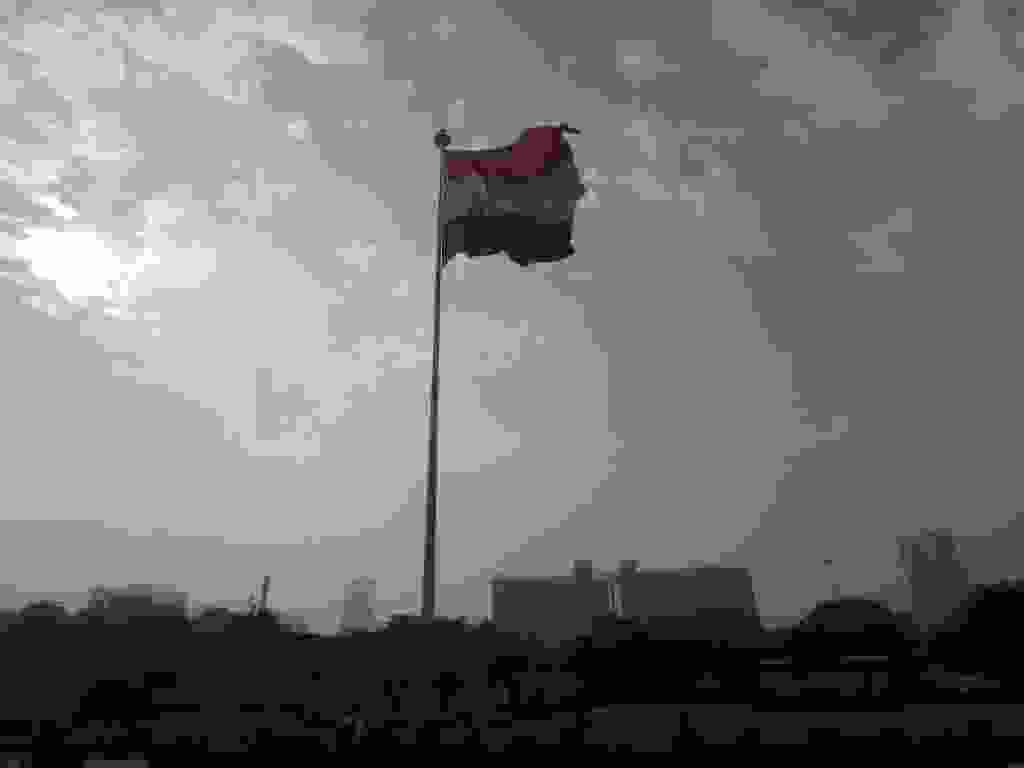
\includegraphics[height=90mm]{../wp-content/uploads/2015/12/wpid-oi0005932-1024x768.jpg} } 
 \newline
 \newline
\centerline{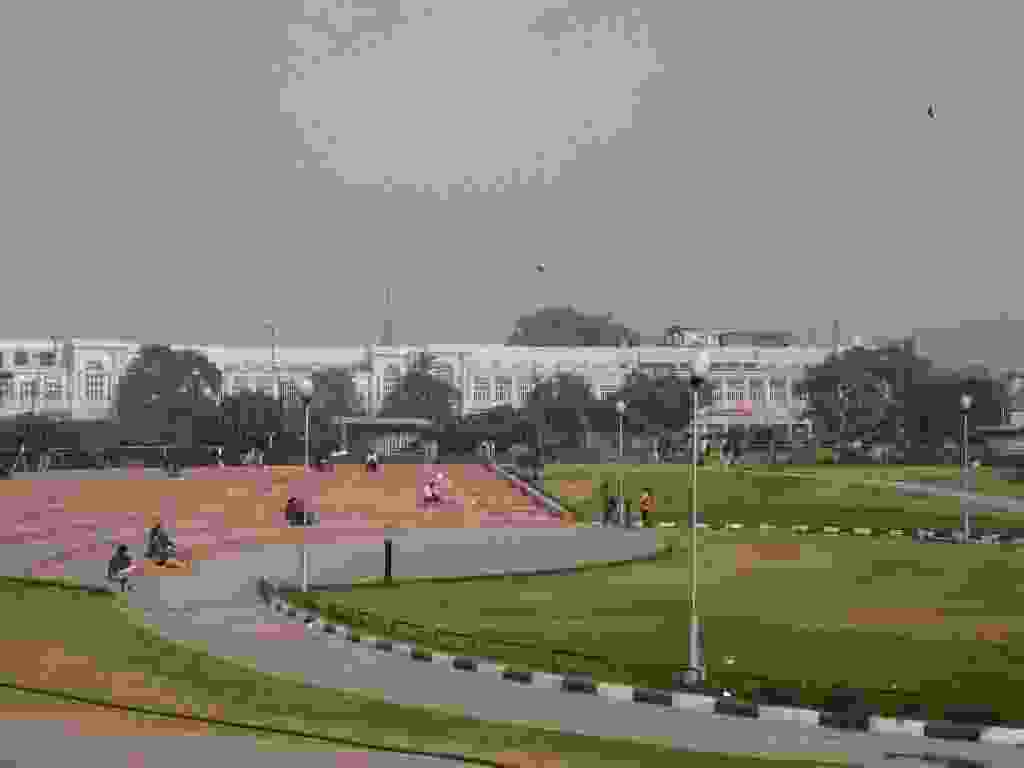
\includegraphics[height=90mm]{../wp-content/uploads/2015/12/wpid-oi0005942-1024x768.jpg} } 
 \newline
 Old Delhi et le Red Fort \newline
 \newline
\centerline{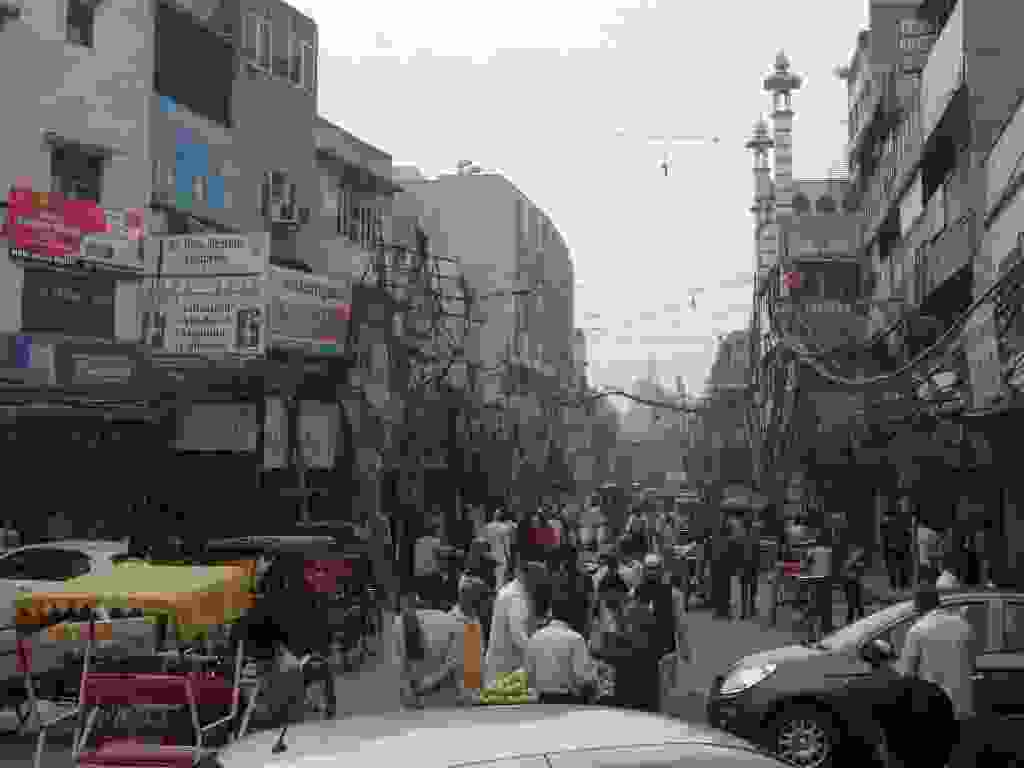
\includegraphics[height=90mm]{../wp-content/uploads/2015/12/wpid-oi0006012-1024x768.jpg} } 
 \newline
 \newline
\centerline{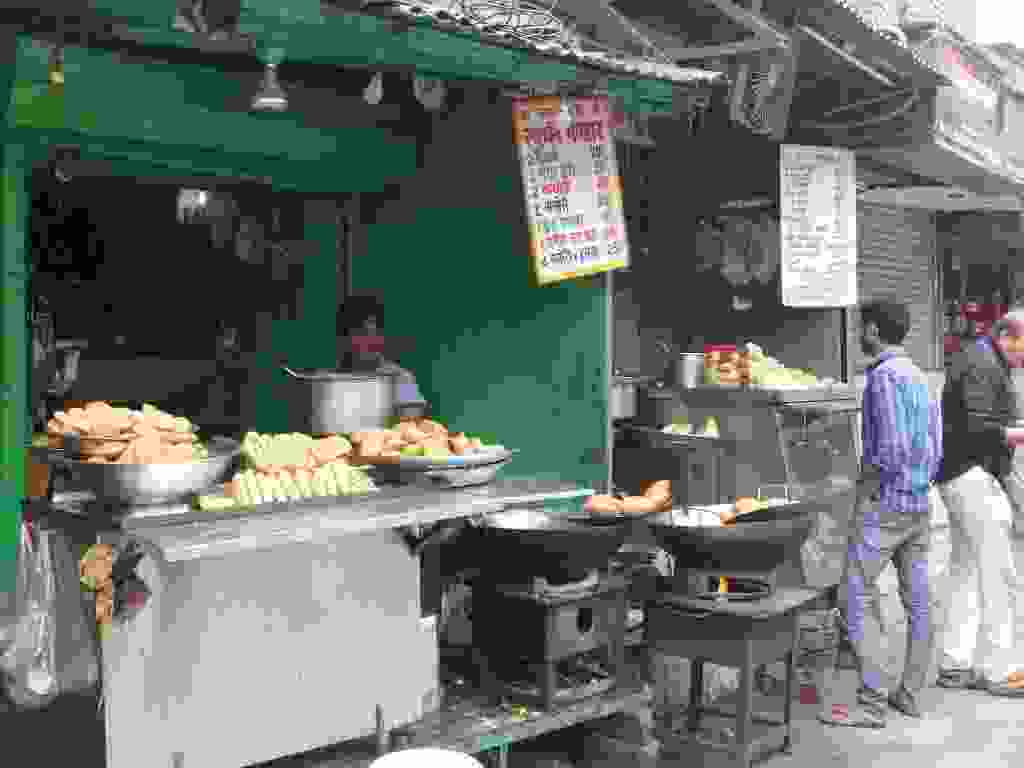
\includegraphics[height=90mm]{../wp-content/uploads/2015/12/wpid-oi0006482-1024x768.jpg} } 
 \newline
 \newline
\centerline{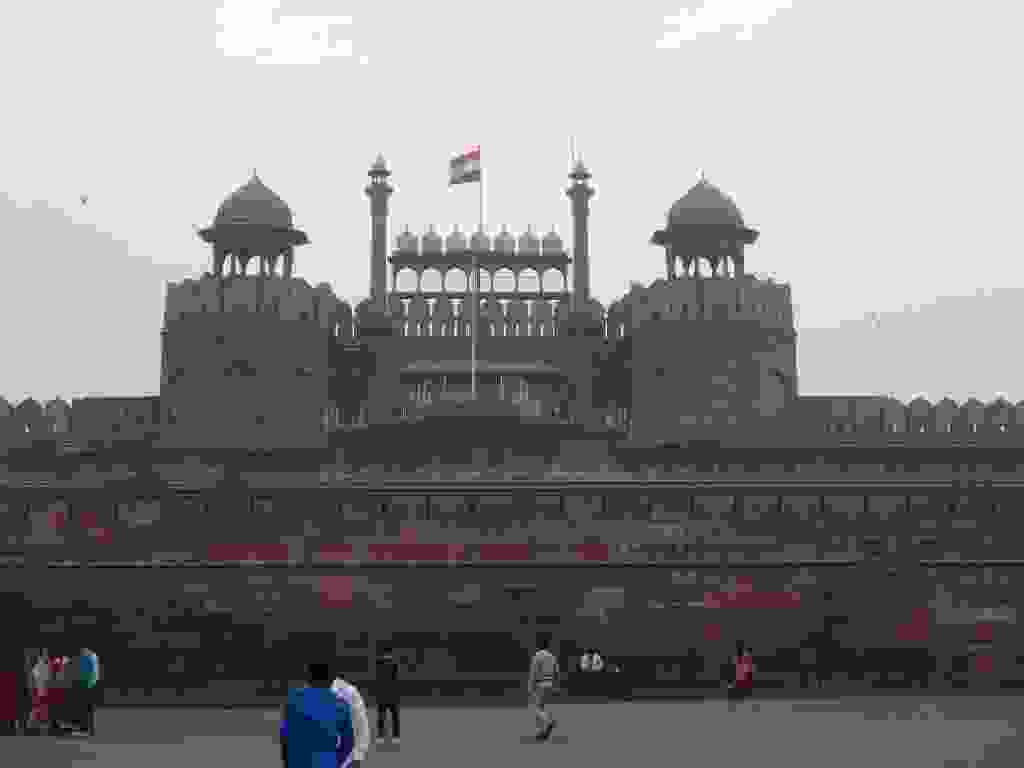
\includegraphics[height=90mm]{../wp-content/uploads/2015/12/wpid-oi0006172-1024x768.jpg} } 
 \newline
 \newline
\centerline{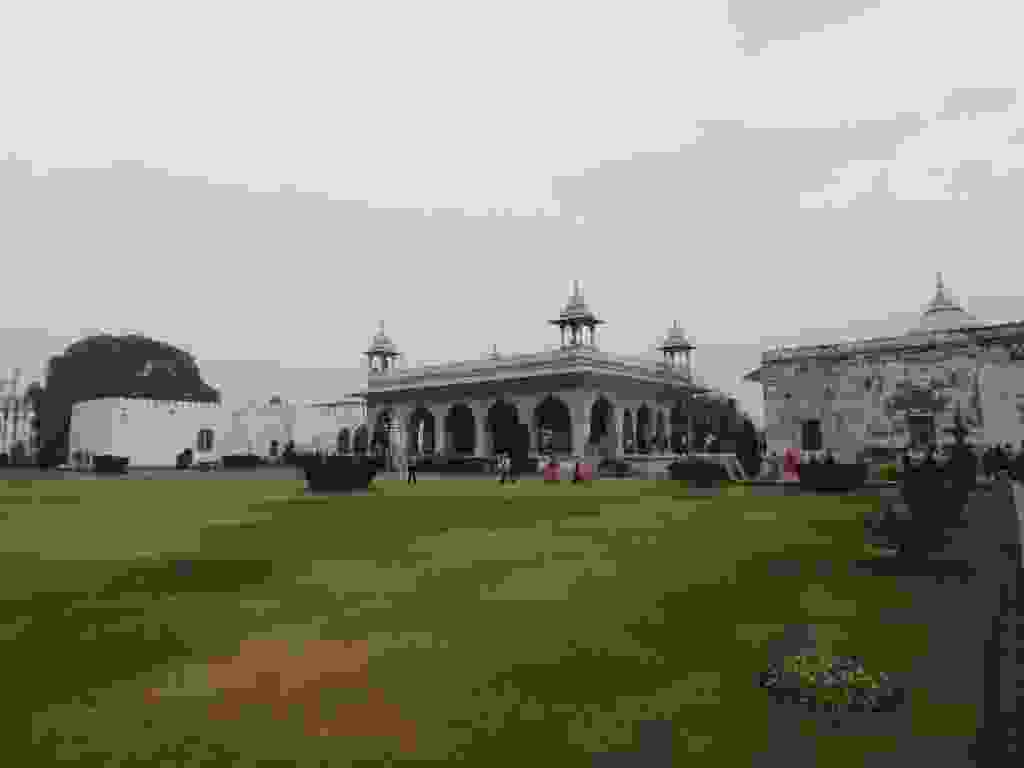
\includegraphics[height=90mm]{../wp-content/uploads/2015/12/wpid-oi0006272-1024x768.jpg} } 
 \newline
 \newline
\centerline{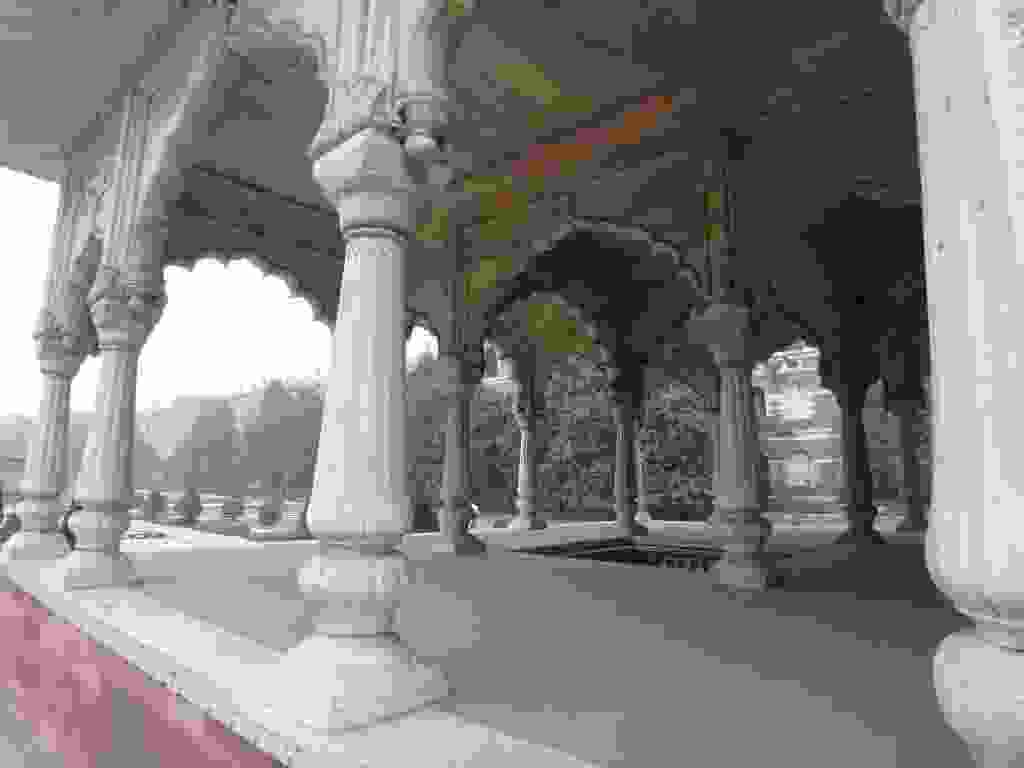
\includegraphics[height=90mm]{../wp-content/uploads/2015/12/wpid-oi0006312-1024x768.jpg} } 
 \newline
 Puis je vais à Meerut où a lieu le mariage : \newline
 Premier jour, c'est la famille du marié qui invite \newline
 Je vais voir la préparation du repas, un grand buffet où on peut goûter à plein de spécialités \newline
 \newline
\centerline{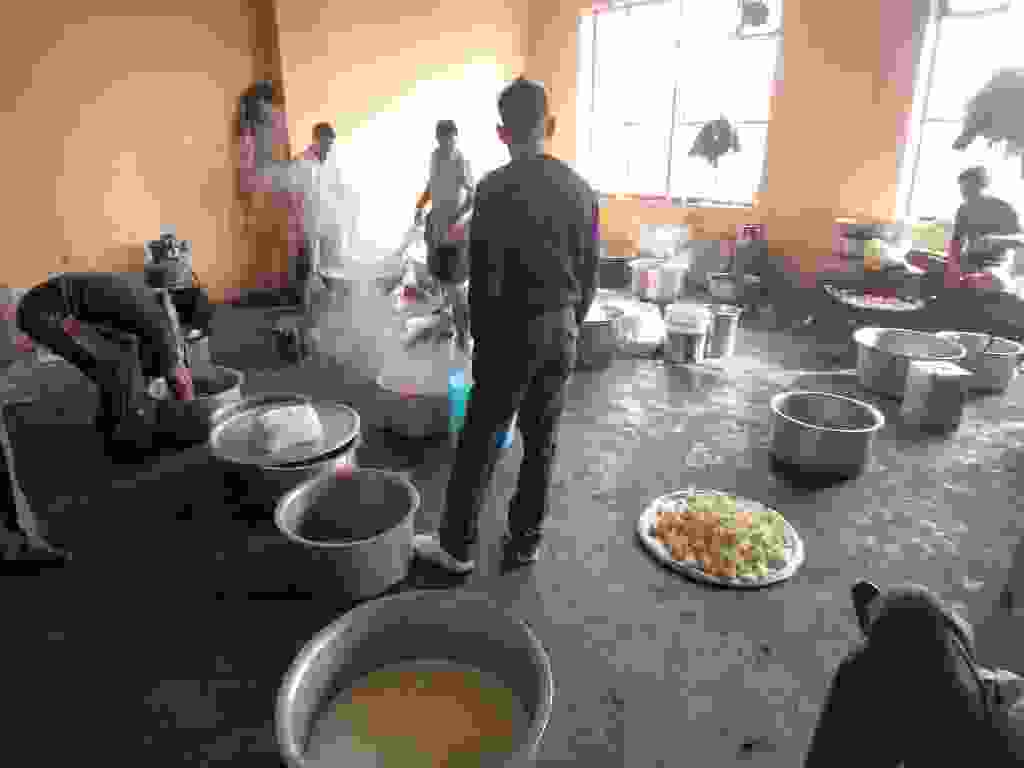
\includegraphics[height=90mm]{../wp-content/uploads/2015/12/wpid-oi0006672-1024x768.jpg} } 
 \newline
 \newline
\centerline{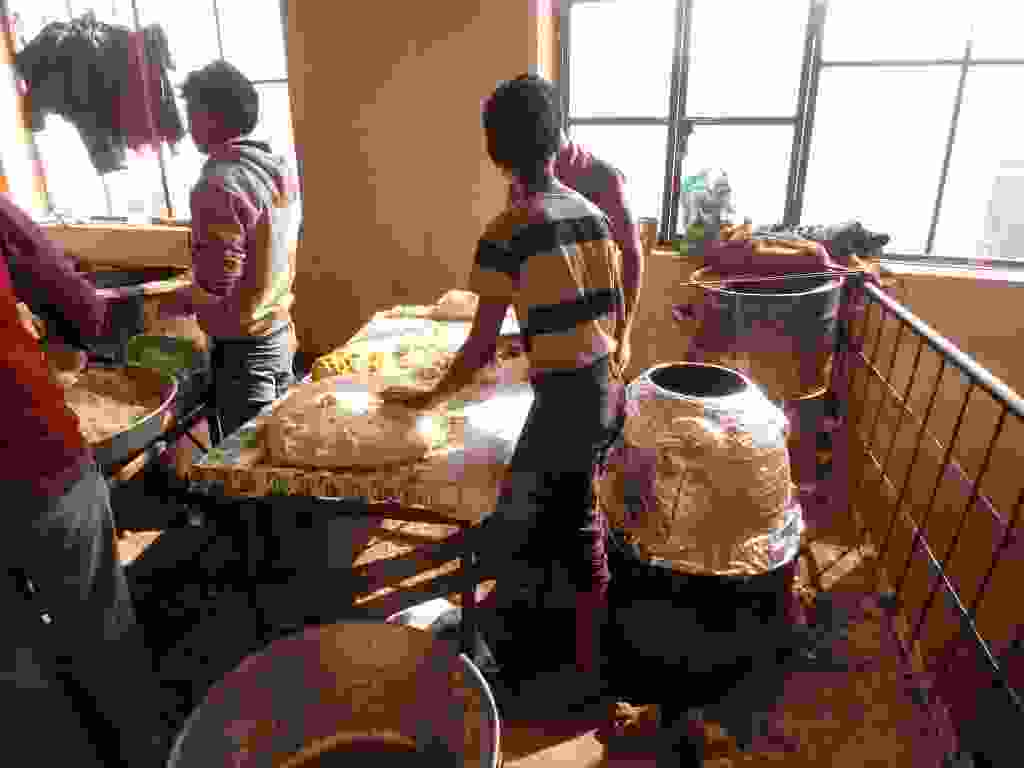
\includegraphics[height=90mm]{../wp-content/uploads/2015/12/wpid-oi0006752-1024x768.jpg} } 
 \newline
 Petite cérémonie avec les 2 familles mais sans la mariée \newline
 \newline
\centerline{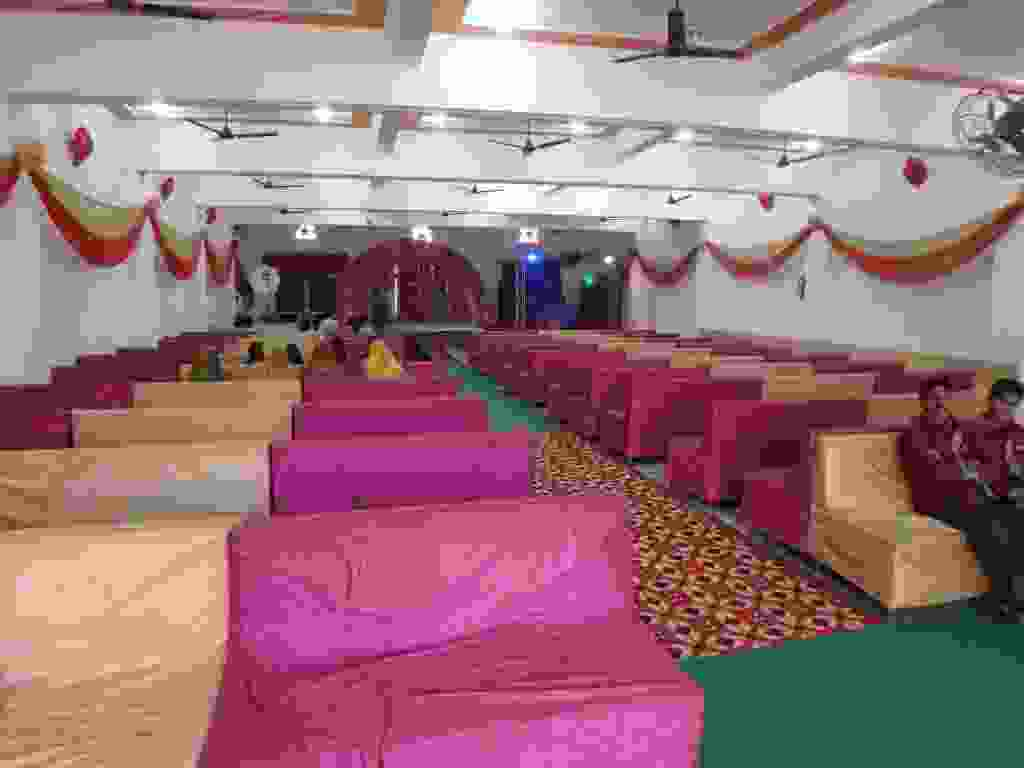
\includegraphics[height=90mm]{../wp-content/uploads/2015/12/OI000685-1024x768.jpg} } 
 \newline
 \newline
\centerline{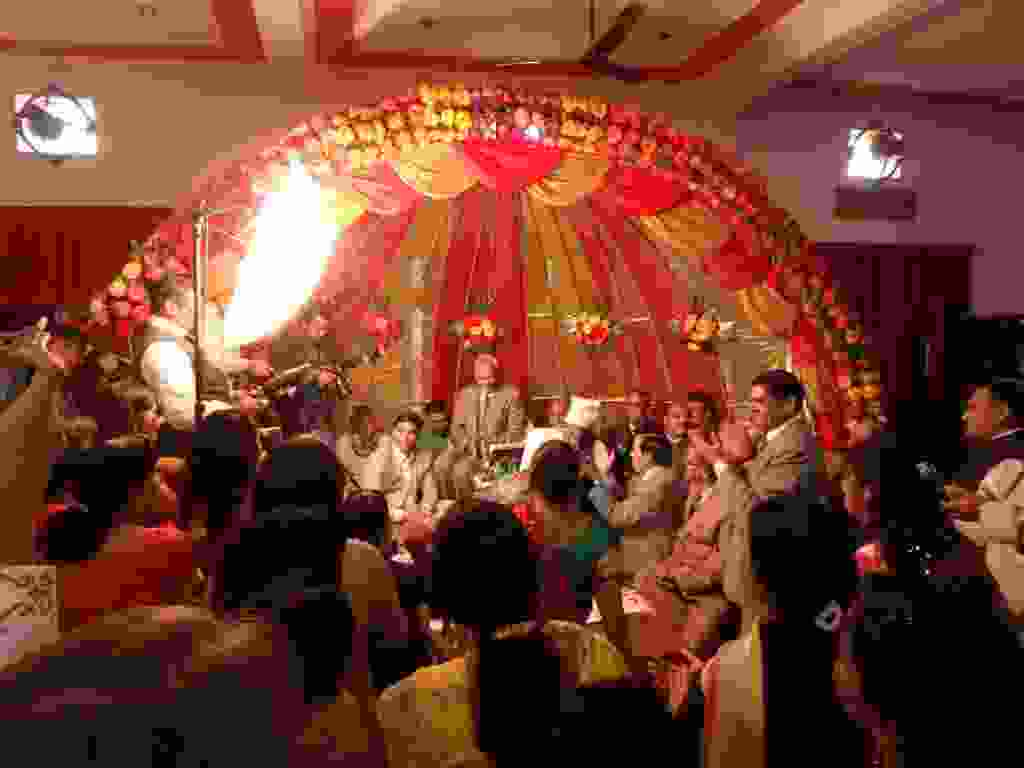
\includegraphics[height=90mm]{../wp-content/uploads/2015/12/wpid-oi0007082-1024x768.jpg} } 
 \newline
 2e jour, rituel où le marié est enduit de curcuma, il ne doit plus sortir de la maison jusqu'au mariage \newline
 \newline
\centerline{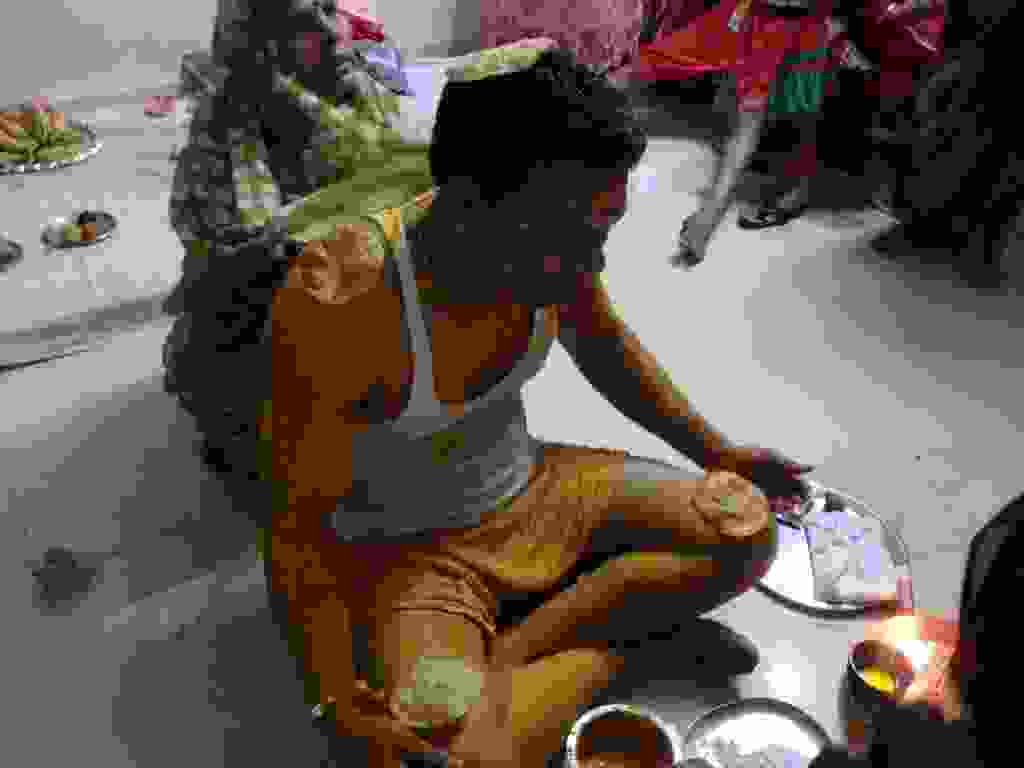
\includegraphics[height=90mm]{../wp-content/uploads/2015/12/wpid-oi000732-1024x768.jpg} } 
 \newline
 Échange de cadeau dans la famille \newline
 \newline
\centerline{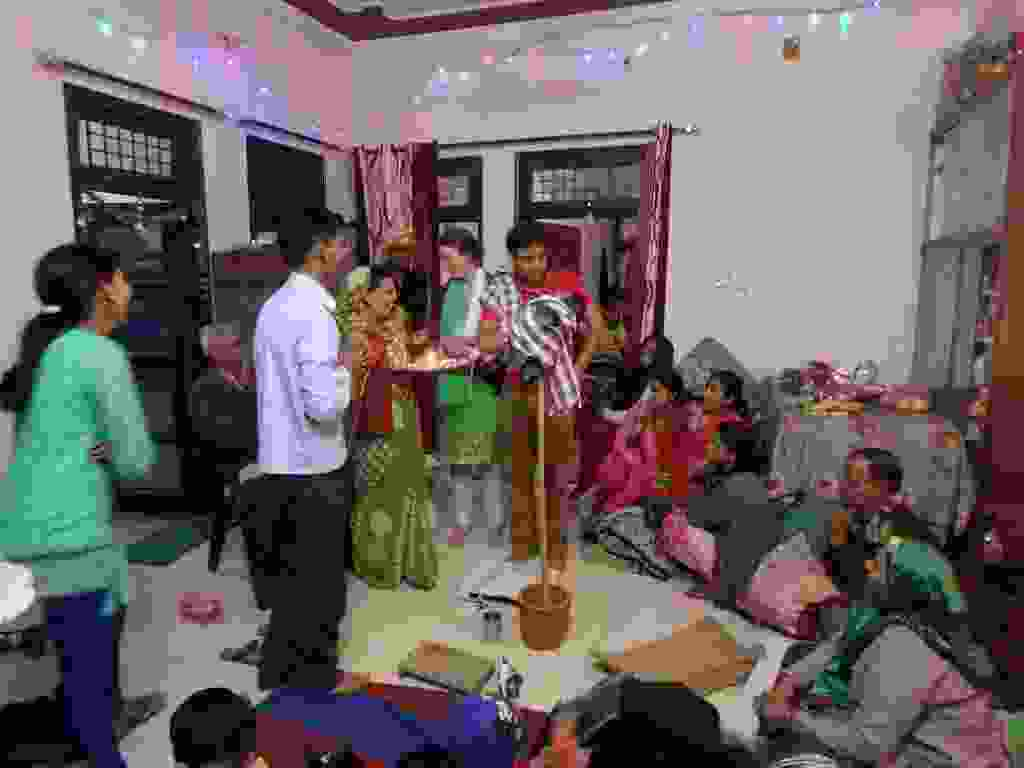
\includegraphics[height=90mm]{../wp-content/uploads/2015/12/wpid-oi000739-1024x768.jpg} } 
 \newline
 3e jour, le vrai mariage \newline
 Préparation du marié \newline
 \newline
\centerline{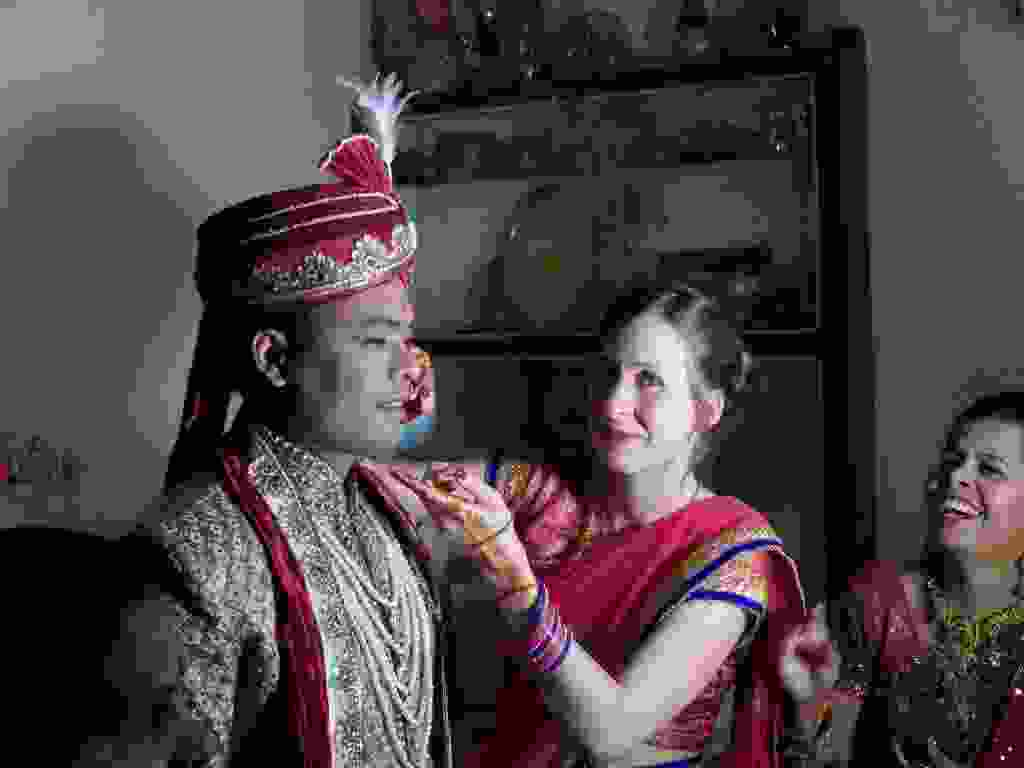
\includegraphics[height=90mm]{../wp-content/uploads/2015/12/wpid-oi000752-1024x768.jpg} } 
 \newline
 Essayage de chapeau, dommage il n'est pas pour moi \newline
 \newline
\centerline{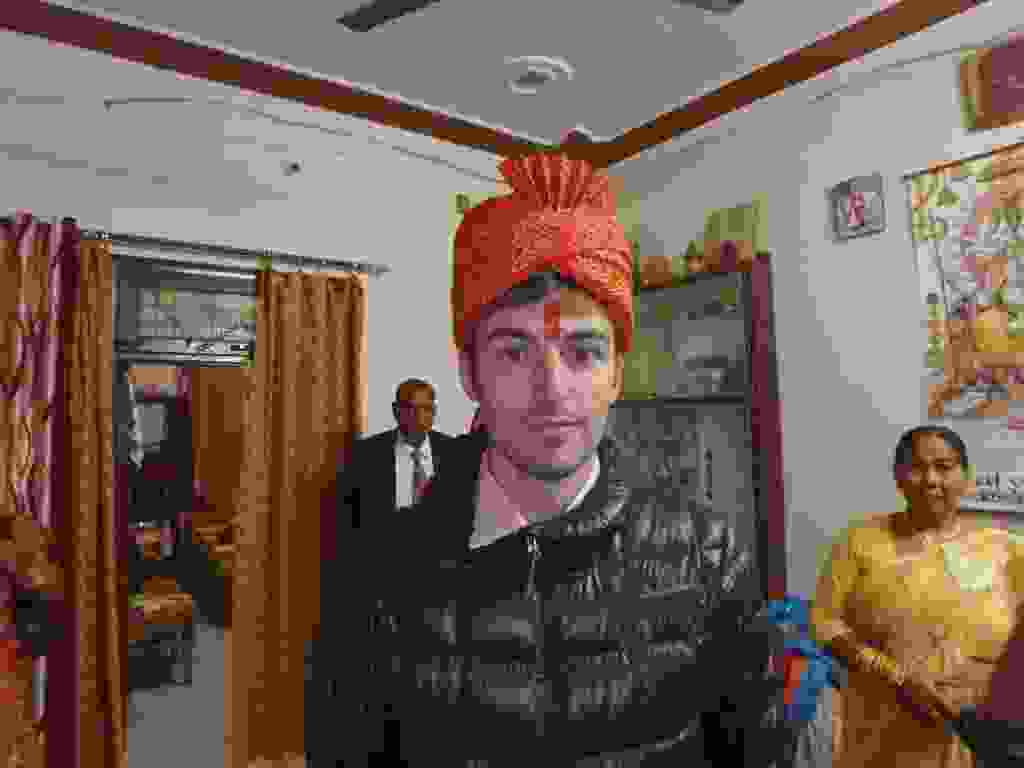
\includegraphics[height=90mm]{../wp-content/uploads/2015/12/wpid-oi000745-1024x768.jpg} } 
 \newline
 Fanfare devant la maison \newline
 \newline
\centerline{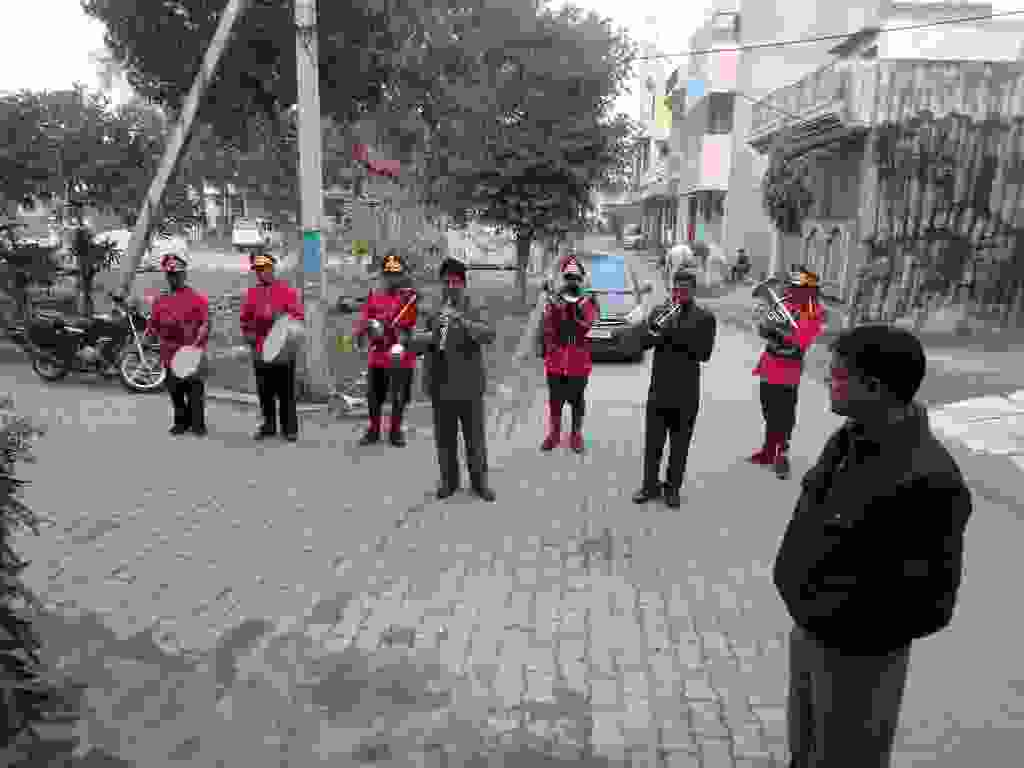
\includegraphics[height=90mm]{../wp-content/uploads/2015/12/wpid-oi0007441-1024x768.jpg} } 
 \newline
 Sortie des 2 frères \newline
 \newline
\centerline{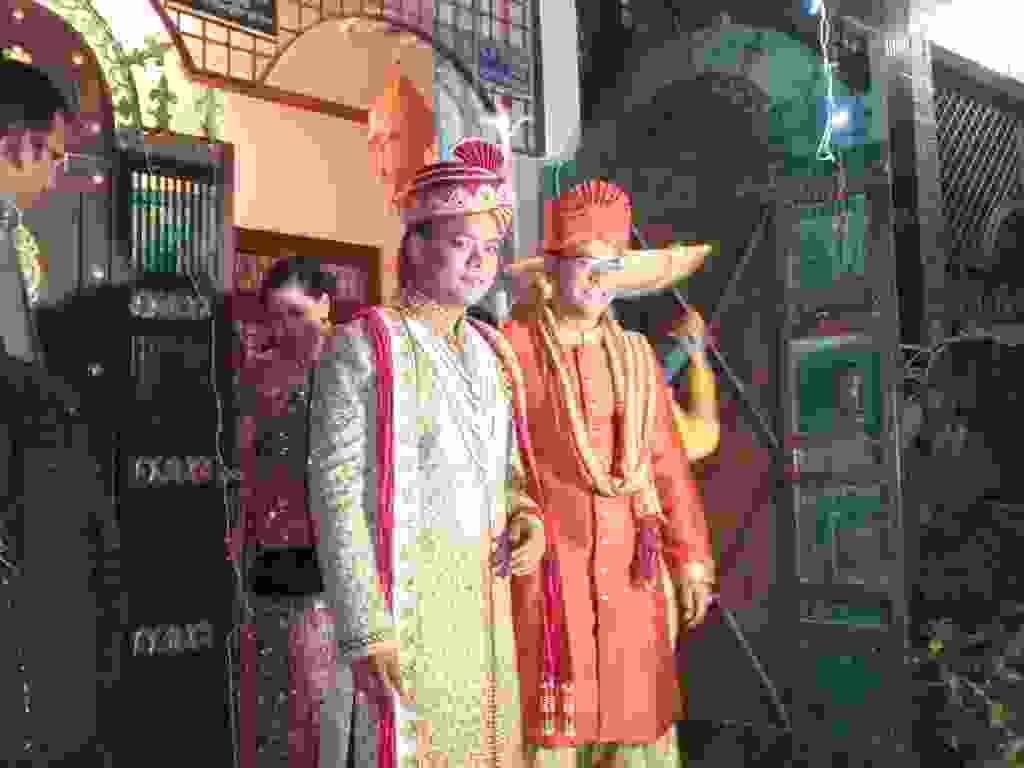
\includegraphics[height=90mm]{../wp-content/uploads/2015/12/wpid-oi000754-1024x768.jpg} } 
 \newline
 On accompagne le marié qui va au temple à cheval \newline
 Puis procession avec toute la famille du marié jusqu'au lieu où la famille de la mariée organise le mariage \newline
 \newline
\centerline{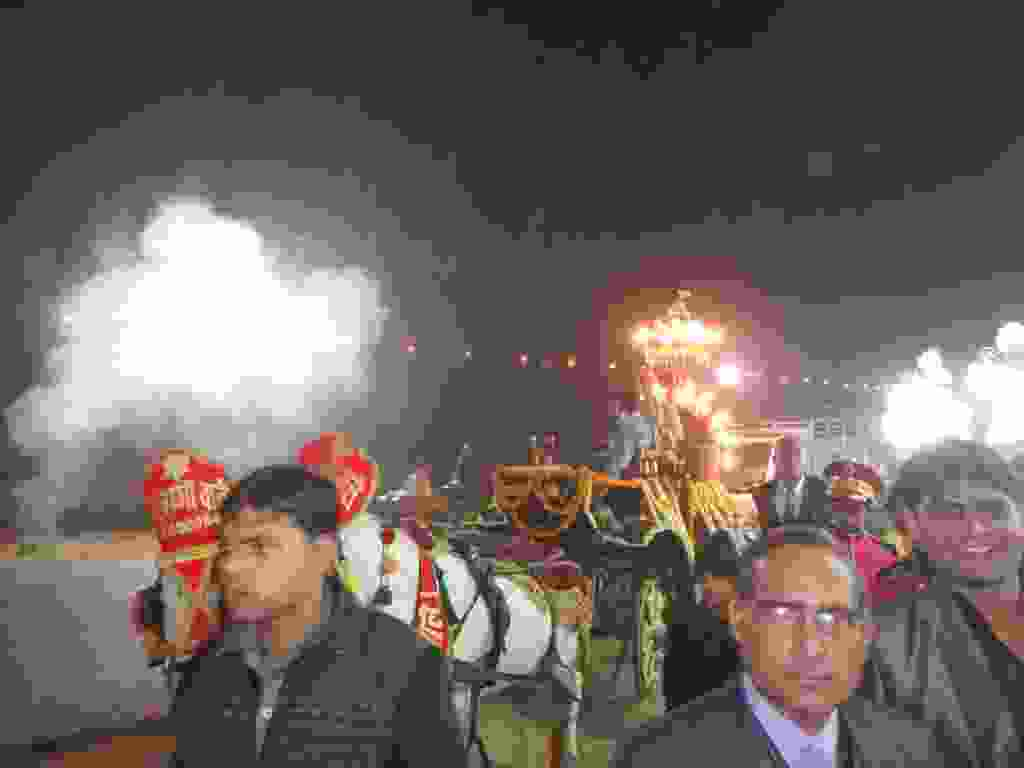
\includegraphics[height=90mm]{../wp-content/uploads/2015/12/wpid-oi000760-1024x768.jpg} } 
 \newline
 \newline
\centerline{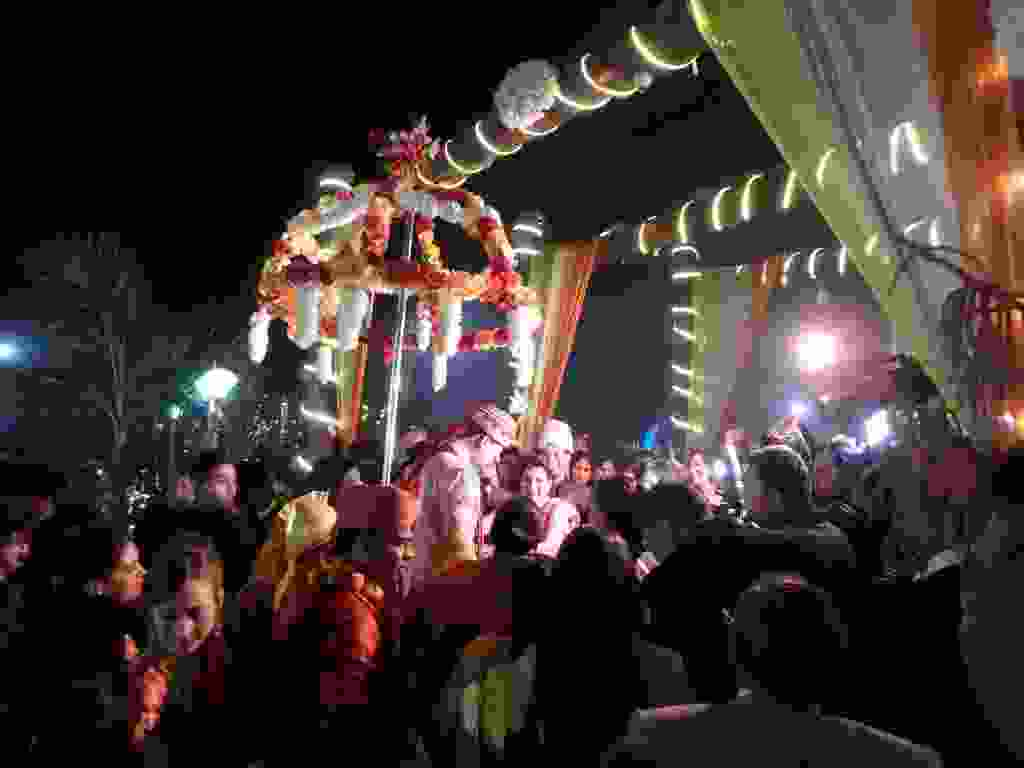
\includegraphics[height=90mm]{../wp-content/uploads/2015/12/wpid-oi000762-1024x768.jpg} } 
 \newline
 \newline
\centerline{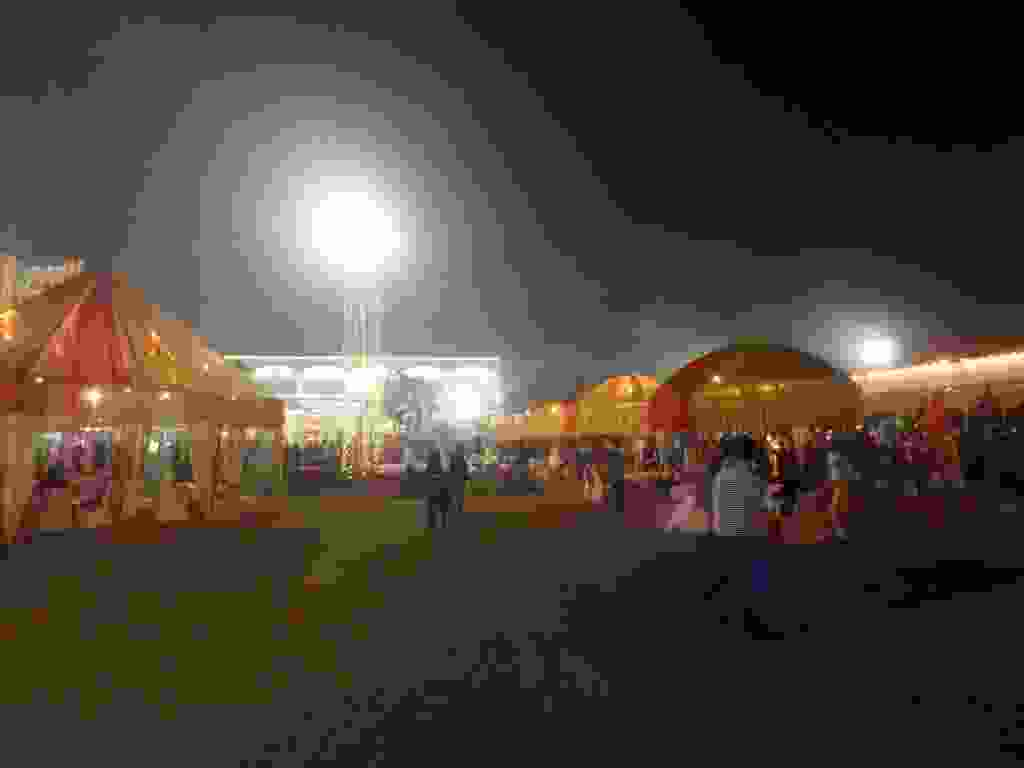
\includegraphics[height=90mm]{../wp-content/uploads/2015/12/wpid-oi000763-1024x768.jpg} } 
 \newline
 Repas encore plus varié que le 1er jour \newline
 \newline
\centerline{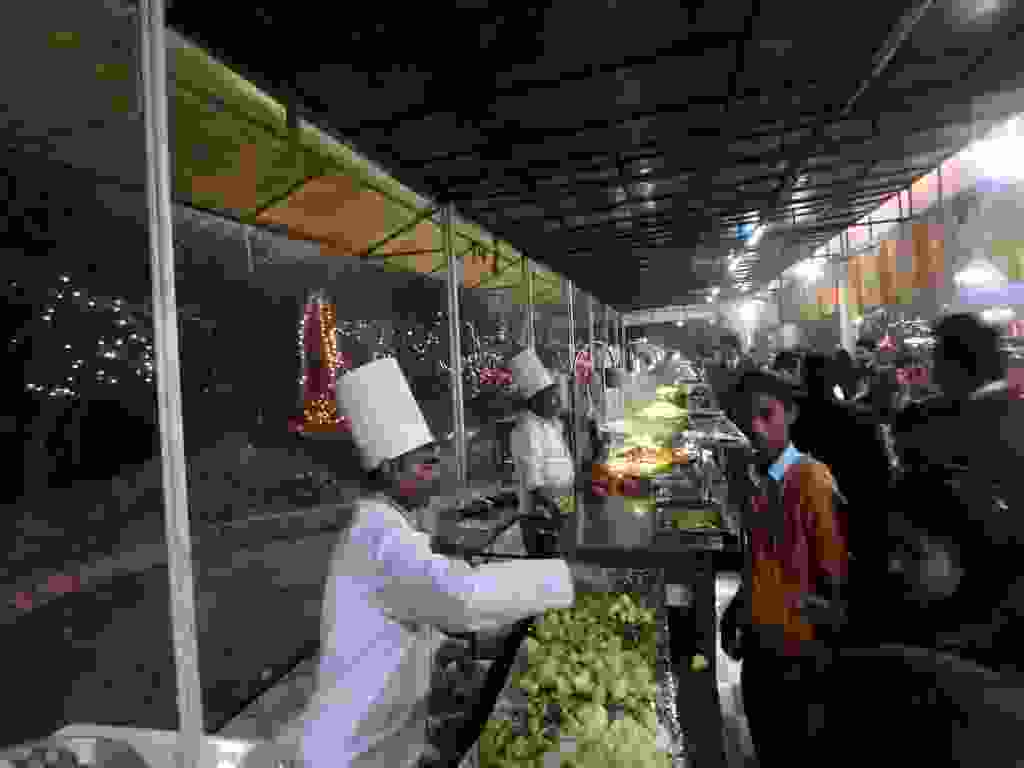
\includegraphics[height=90mm]{../wp-content/uploads/2015/12/wpid-oi000766-1024x768.jpg} } 
 \newline
 Séance photo, quasiment tous les invités passent, ça fait quelques centaines de personnes \newline
 \newline
\centerline{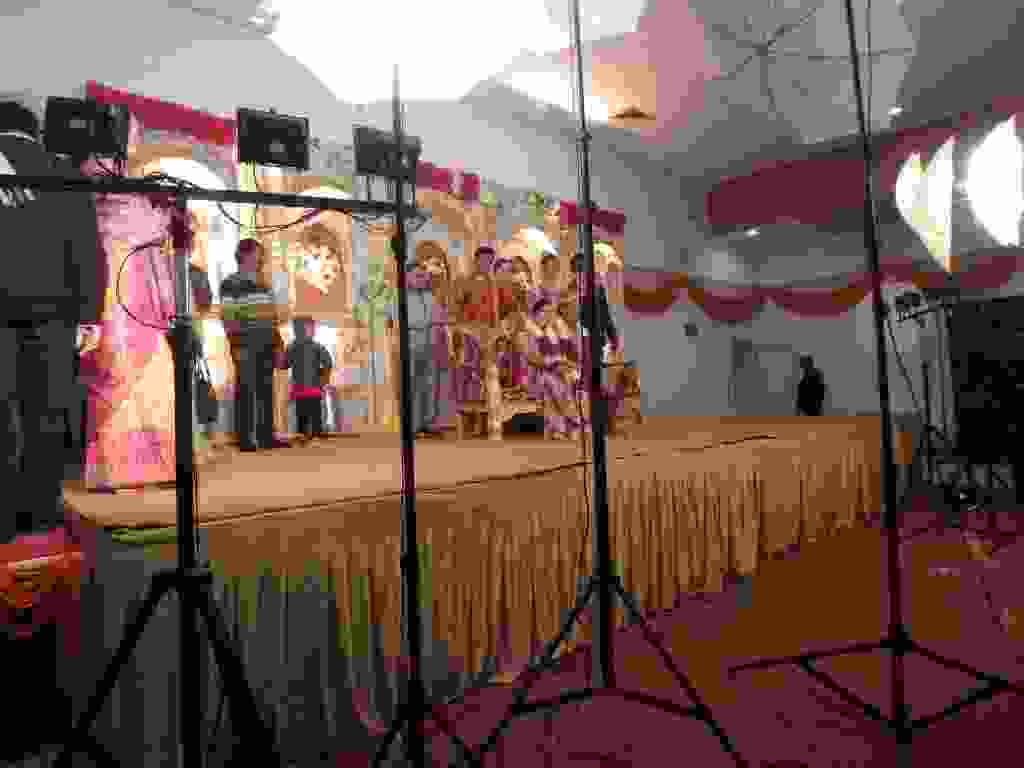
\includegraphics[height=90mm]{../wp-content/uploads/2015/12/wpid-oi000774-1024x768.jpg} } 
 \newline
 Enfin cérémonie autour d'un feu avec le prêtre hindou, entre 2h et 4h du matin \newline
 \newline
\centerline{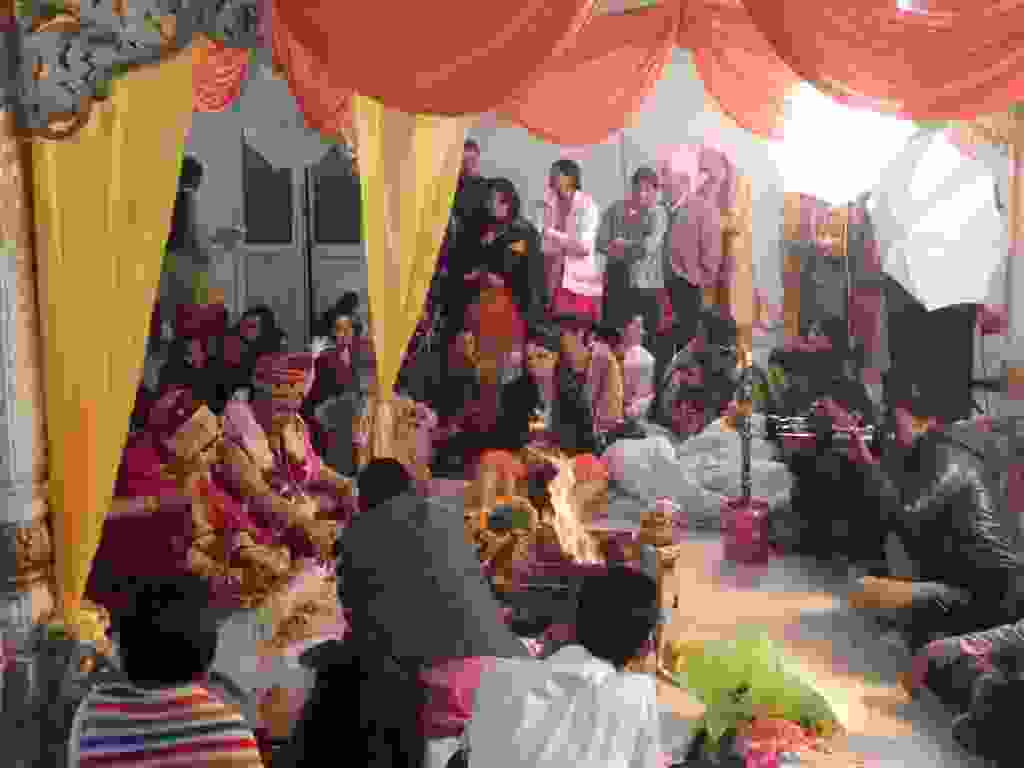
\includegraphics[height=90mm]{../wp-content/uploads/2015/12/wpid-oi000783-1024x768.jpg} } 
 \newline

\newpage
 
